%\documentclass{selecciones}% DESCOMENTAR SI USA OVERLAG 
%\documentclass[leqno]{Base/Selecciones}
	\documentclass{Base/Selecciones}
%%%%%%%%%%%%%%%%%%%%%%%%%%%%%%%%%%%%%%%%%%%%%%%%%%%%%%%%%%%%%%                             MARGENES                               %%%%%%%%%%%%%%%%%%%%%%%%%%%%%%%%%%%%%%%%%%%%%%%%%%%%%%%%%%%
\marginsize{3cm}{3cm}{1cm}{2.5cm}  % Márgenes del documento
%\usepackage[hmarginratio=1:1,top=25mm,bottom=20mm,left=25mm,right=25mm,columnsep=20pt]{geometry}
%%%%%%%%%%%%%%%%%%%%%%%%%%%%%%%%%%%%%%%%%%%%%%%%%%%%%%%%%%%%%%
%                IDIOMA, CODIFICACION & FUENTES              %
%%%%%%%%%%%%%%%%%%%%%%%%%%%%%%%%%%%%%%%%%%%%%%%%%%%%%%%%%%%%%%
\usepackage[spanish,USenglish,brazil,es-tabla]{babel}  % 
%\usepackage[brazil]{babel}  % Habilitar para el artículos en portugués
%\usepackage[spanish, es-tabla]{babel}  % Habilitar para el caso de tablas en español
%\usepackage[latin1]{inputenc}
\usepackage[utf8]{inputenc}
\usepackage{mathrsfs}
\usepackage{amsmath}
\usepackage{amstext}
\usepackage{amsfonts}
\usepackage{marvosym}
\usepackage[psamsfonts]{amssymb}
\usepackage{latexsym}
\usepackage{bm}

%%%%%%%%%%%%%%%%%%%%%%%%%%%%%%%%%%%%%%%%%%%%%%%%%%%%%%%%%%%%%%%%%%%%%%
%                     IMAGENES, COLOR & GRAFICOS                     %
%%%%%%%%%%%%%%%%%%%%%%%%%%%%%%%%%%%%%%%%%%%%%%%%%%%%%%%%%%%%%%%%%%%%%%
%\usepackage{graphicx} % figuras
%\usepackage{subfig}
\usepackage{rotating}
\usepackage[dvips,final]{epsfig}
\usepackage{colortbl}
\usepackage{color}
\usepackage[light]{draftcopy}
\usepackage{pgfkeys}
%\usepackage{texdraw}
\usepackage{pgf}
\usepackage{pgfplots}
	\pgfplotsset{compat=1.13}
\usepackage{pgfplotstable}
\usepackage[all]{xy}
%\usepackage[caption=false]{subfig}
\usepackage{pst-node}
	\usetikzlibrary{fadings}
	\usetikzlibrary{positioning,shapes,fit,arrows}
	\usetikzlibrary{mindmap,trees}
	\usetikzlibrary{shadows}
	\usetikzlibrary{shapes,arrows,calc,intersections}
	\usetikzlibrary{decorations.markings}
	\usetikzlibrary{decorations.pathreplacing}
%\usepackage{caption}
%\usepackage{lipsum}  % Para crear texto de relleno
%%%% %%%%%%%%%%%%%%%%%%%%%%%%%%%%%
%		subfigures													
%%%%%%%%%%%%%%%%%%%%%%%%%%%%%%%%%
\usepackage{caption}
\usepackage{subcaption}
%%%%%%%%%%%%%%%%%%%%%%%%%%%%%%%%%%%%%%%%%%%%%%%%%%%%%%%%%%%%%%%%%%%%%%
%                            REFERENCIAS                             %
%%%%%%%%%%%%%%%%%%%%%%%%%%%%%%%%%%%%%%%%%%%%%%%%%%%%%%%%%%%%%%%%%%%%%%
\usepackage{varioref}
\usepackage[pagewise]{lineno}\linenumbers
\usepackage[colorlinks=true,citecolor=red,linkcolor=blue,urlcolor=cyan,filecolor=magenta]{hyperref}
\usepackage{fancyhdr}
%%%%%%%%%%%%%%%%%%%%%%%%%%%%%%%%%%%%%%%%%%%%%%%%%%%%%%%%%%%%%%%%%%%%%%
%                              TABLAS                                %
%%%%%%%%%%%%%%%%%%%%%%%%%%%%%%%%%%%%%%%%%%%%%%%%%%%%%%%%%%%%%%%%%%%%%%
\usepackage{array,float} % para usar [H]
\usepackage{multirow,multicol}
\usepackage{longtable}
\usepackage{csvsimple}
\usepackage{lscape}
%%%%%%%%%%%%%%%%%%%%%%%%%%%%%%%%%%%%%%%%%%%%%%%%%%%%%%%%%%%%%%%%%%%%%%
%                     ALGORITMOS Y PSEUDOCODIGO                      %
%%%%%%%%%%%%%%%%%%%%%%%%%%%%%%%%%%%%%%%%%%%%%%%%%%%%%%%%%%%%%%%%%%%%%%
\usepackage{algpseudocode}
\usepackage{algorithm} %%%%%%%%%UM MOMENTO
\usepackage{listings}

%%%%%%%%%%%%%%%%%%%%%%%%%%%%%%%%%%%%%%%%%%%%%%%%%%%%%%%%%%%%%%%%%%%%%%
%                               OTROS                                %
%%%%%%%%%%%%%%%%%%%%%%%%%%%%%%%%%%%%%%%%%%%%%%%%%%%%%%%%%%%%%%%%%%%%%%
\usepackage{appendix}
\graphicspath{{IMG/ART1/}}

%============================================================%
%                          MACROS                            %
%============================================================%



%============================================================%
%                       CONFIGURACION                        %
%============================================================%

%\previewtrue
%\communicationtrue

\title{A mathematical model of obesity % (es OBLIGATORIO)
	\\
	%
	\vspace{0.4cm}
	%
	%{Un modelo matemático de la obesidad } % (SI EL ARTICULO ES EN INGLES EL TITULO EN ESPAÑOL ES OPCIONAL)
}

% Fill in the data of the authors and then comment them
\autor{}{}{}
%\autor{Soledad Quiróz  Lugo}
%	{https://orcid.org/0000-0002-7703-5781}
%	{Instituto de Investigaciones,  Universidad de Puebla, Puebla, México ({\tt slepe@upuebla.edu.pe}).}
%	\and 
%\autor{Jaime Reyes }
%	{https://orcid.org/0000-0002-7000-548}
%	{Departamento de Matemáticas,  Universidad Nacional de Trujillo, Trujillo, Perú ({\tt reyesj@unitru.edu.pe}).}





\edition{2020}{7(1)}{1}{9}  % Edición del artículo

%\received{Feb. 22, 2020}

%\accepted{Apr. 30, 2020}

%\public{ jun. 20, 2024}

%\doi{http://dx.doi.org/10.17268/sel.mat.2020.01.01}

%\howtocite{López R.}{Un modelo matemático-epidemiológico del control de la obesidad}


%============================================================%
%                         DOCUMENTO                          %
%============================================================%
\begin{document}

\maketitle
\begin{center}
\textcolor{red}{\large \bf Special Issue: Workshop on Optimization and Operator Learning - SaC3 - Perú}	
\end{center}
\vspace{1cm}
	
	%
%	\headertext % Encabezado de cada pagina

\selectlanguage{USenglish}

%--------------------------------------------------------------
	\begin{remark*}
	\textcolor{gray}{
	The TITLE and ABSTRACT is Mandatory. moreover, if the manuscript is written in Spanish add  RESUMEN o in Portuguese add RESUMO.} 
	\end{remark*}	

	%--------------------------------------------------------------

\bigskip 
	%%%%%%%%%%%%%%%%%%%%%%%%%%%%%%%%%%%%%%%%%%%%%%%%%%%%%%%%%%%%%%%%%%
	%                       ABSTRACT EN INGLES ( Mandatory-  OBLIGATORIO)                       %
	%%%%%%%%%%%%%%%%%%%%%%%%%%%%%%%%%%%%%%%%%%%%%%%%%%%%%%%%%%%%%%%%%%
	\selectlanguage{USenglish}  % Select the language English
	%( if prefer other language select your language ) and write
	\begin{abstract}
		In this work, the work is investigated and presented precisely, indicating the new contribution of knowledge, the latter is important, because if it is not, it runs the risk of not being accepted.
	\end{abstract}
	
	\begin{keywords}
		Ordinary differential equation, multilevel, Stability, Simulation.
	\end{keywords}

	
	%%%%%%%%%%%%%%%%%%%%%%%%%%%%%%%%%%%%%%%%%%%%%%%%%%%%%%%%%%%%%%%%%%
	%                       RESUMEN EN ESPAÑOL ( Solo Si el Manuscrito es escrito en ESPAÑOL )                      %
	%%%%%%%%%%%%%%%%%%%%%%%%%%%%%%%%%%%%%%%%%%%%%%%%%%%%%%%%%%%%%%%%%%
	%\selectlanguage{spanish}  % Seleccionamos el idioma español
	
	%\begin{abstract}
%		En este trabajo,  se investiga y se presenta el trabajo de manera precisa , indicando la contribución nueva del conocimiento, es importante esto último, porque si no es así, corre el riesgo de de no ser aceptado.
%	\end{abstract}
	
%	\begin{keywords}
%		Ecuación diferencial ordinaria, muĺtiple nivel,  estabilidad, simulaci\'on.
%	\end{keywords}
	

	
	%%%%%%%%%%%%%%%%%%%%%%%%%%%%%%%%%%%%%%%%%%%%%%%%%%%%%%%%%%%%%%%%%%
	%                       RESUMO EM PORTUGUES  (SOMENTE se o manuscrito estiver escrito em PORTUGUÊS )                       %
	%%%%%%%%%%%%%%%%%%%%%%%%%%%%%%%%%%%%%%%%%%%%%%%%%%%%%%%%%%%%%%%%%%
	%\selectlanguage{brazil}  % Selecciona o lengua portugues
	
	%\begin{abstract}
%	Neste trabalho, o trabalho é investigado e apresentado de forma precisa, indicando a nova contribuição do conhecimento, este último é importante, pois se assim não for, corre-se o risco de não ser aceito. 
%	\end{abstract}
	
%	\begin{keywords}
%		Equação diferencial ordinária, nível múltiplo, estabilidade, simulação. 
%	\end{keywords}	
	
	
	
	%%%%%%%%%%%%%%%%%%%%%%%%%%%%%%%%%%%%%%%%%%%%%%%%%%%%%%%%%%%%%%%%%%
	%                           SECCIONES                            %
	%%%%%%%%%%%%%%%%%%%%%%%%%%%%%%%%%%%%%%%%%%%%%%%%%%%%%%%%%%%%%%%%%%
	
%	\selectlanguage{spanish} % Si el Documento es en español , seleccione <espanish>, en Portugues seleciones <brazil> si esn en inglés use \selectlanguage{USenglish}

	
	\section{Introduction}

	

	In the universal literature on mathematical modeling of obesity, there are two aspects of its study, one from the epidemiological point of view, since due to poor eating habits or physical activity, these have been propagation factors in the diverse populations of this chronic disease, obesity ( population-based model) as in \cite{ar}, \cite{ev} and the other point of view is physiological in terms of the type of food consumed (individual-based model) \cite{ff}\cite{lo}.

	

	\section{Model}
	For the construction of this model, we will consider three subpopulations of the total population, individuals with normal weight $N(t)$, individuals with overweight $S(t)$ and those individuals who are obese $O(t)$. Let's also consider some assumptions:



	\medskip
	%\begin{itemize}	
	%	\item La población total es homogénea, es decir tiene condiciones de salud similares.
		
	%	\item Las personas pasan a las diferentes etapas de peso no normal por el consumo excesivo de comida no sana (harinas, frituras, bebidas gaseosas).
	%\end{itemize}

%	\medskip
	The transitions between these three subpopulations occur as follows:
%	\medskip
	\begin{itemize}
		\item A person of normal weight $N(t)$ who begins to overindulge in unhealthy food begins his transition to an overweight person $S(t)$.
		
		\item An overweight person S(t) who continues with his excess of unhealthy food, becomes a person with obesity O(t).
		
		\item ...
		\item ...
	\end{itemize}

	\medskip
	With all these considerations, the model is (see in
	 \cite{th})

	\begin{equation}
		\begin{array}{ccl}
			{\displaystyle \frac{dN(t)}{dt}}&=&(1-\rho)\mu P(t) -\alpha  {\displaystyle\frac{S(t)}{P(t)}}N(t) - \beta {\displaystyle\frac{O(t)}{P(t)}}N(t)-\mu N(t)\\
			{\displaystyle\frac{dS(t)}{dt}}&=&\rho\mu P(t) +\alpha {\displaystyle\frac{S(t)}{P(t)}}N(t)-(\epsilon + \mu) S(t)\\
			{\displaystyle\frac{dO(t)}{dt}}&=& \beta {\displaystyle\frac{O(t)}{P(t)}}N(t)+\epsilon S(t)-\mu O(t)
		\end{array}
		\label{eq:1}
	\end{equation}
	
	where the variables for the basic model are given in Table \ref{ta:1}
	\begin{table}[htb]
		\centering
		\begin{tabular}{|c|l|}
			\hline
			%
			{\bf Variables} & {\bf Meaning} \\
			%& \\
			\hline
			% & \\
			$N(t)$ &Non-obese population at any time t (people with IMC less than 24.9)\\
			%& \\
			\hline
			%& \\
			$S(t)$ & Overweight non-obese population at any time t (people starting to \\
& eat calories, i.e. with IMC between 25 and 29.9)\\
			%& \\
			\hline
			% & \\
			$O(t)$ & Obese population at any time t (people with IMC greater than 30)\\
			%& \\
			\hline
			% & \\
			$P(t)$ & Total population at any time $t$,
			$P(t)=N(t)+S(t)+O(t)$
			\\
			%& \\
			\hline
		\end{tabular}
		\caption{System Variable Meanings (\ref{eq:1})}
		\label{ta:1}
	\end{table}


	\subsection{System Reduction} 
	
	
	When using sufigures, we have to use the following format
%	
	
	\begin{figure}[!tbp]
  \begin{subfigure}[b]{0.22\textwidth}
    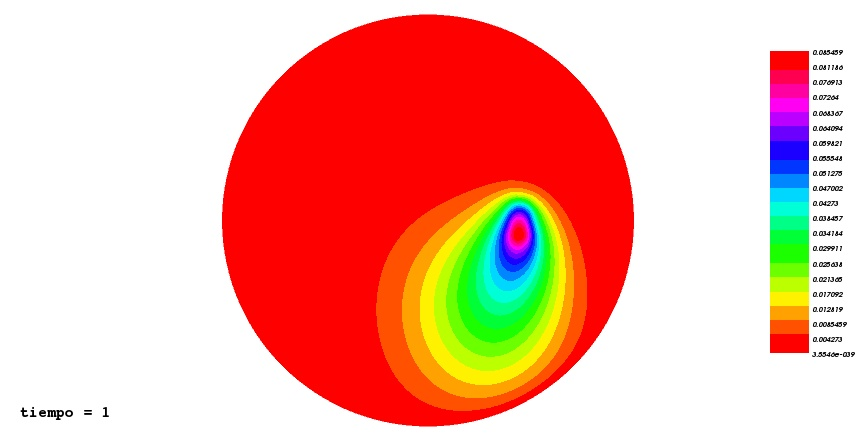
\includegraphics[width=\textwidth, height=\textwidth]{b1}
    \caption{Primera imagen.}
    \label{fig:f1}
  \end{subfigure}
  \qquad
  \begin{subfigure}[b]{0.22\textwidth}
    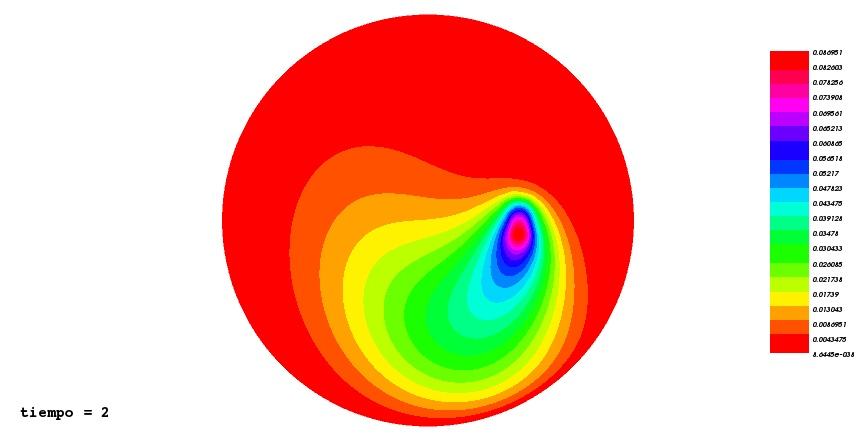
\includegraphics[width=\textwidth, height=\textwidth]{b2}
    \caption{Primera imagen.}
    \label{fig:f1}
  \end{subfigure}\qquad 
  \begin{subfigure}[b]{0.22\textwidth}
    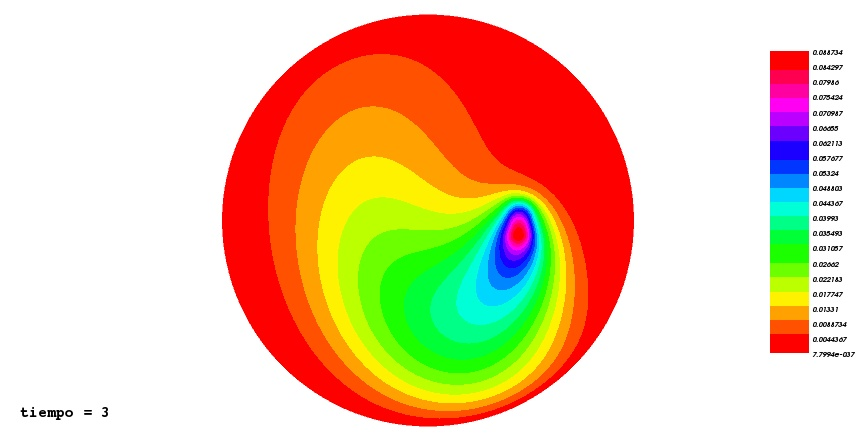
\includegraphics[width=\textwidth, height=\textwidth]{b3}
    \caption{Segunda imagen.}
    \label{fig:f2}
  \end{subfigure}
  \caption{Dos imágenes en la misma figura.}
\end{figure}
	
	
	
		Consequently, the system (\ref{eq:1}) is reduced to the study of a Normalized two-dimensional system,
		% consideramos las subpoblaciones $s(t)=  {\displaystyle{S(t)}{P}}$ y $o(t)=  {\displaystyle{O(t)}{P}}$, 
		
		\begin{equation}
			\begin{array}{ccl}
				{\displaystyle\frac{ds}{dt}}&=&\rho\mu +\alpha  s[1-(s+o)]-(\epsilon + \mu) s\\
				{\displaystyle\frac{do}{dt}}&=& \beta o[1-(s+o)]+\epsilon s-\mu o
			\end{array}
			\label{eq:3}
		\end{equation}
	
	\medskip
	\subsection{Model Analysis}
Existence of solutions;

		\begin{theorem}
			For all $s_0,o_0>0$ , exist $s,o:[0,\infty)\longrightarrow[0,\infty)$ that solve the system (\ref{eq:3}) with initial conditions $s=s_0,o= o_0$.

			 Also. All solutions of the system (\ref{eq:3}) are bounded and positive.
		\end{theorem}

		\begin{proof}
			The existence of the solutions is guaranteed by Peano's theorem.
			... \squareproof
		\end{proof}





	\subsection{Simulations}
	
	Here is a simulation of the obesity model given by (\ref{eq:1}), with initial conditions dating from the year 2005 $(t=0)$. % until the year where the values of the initial conditions are given in Table \ref{ta:3}

	%\begin{table}[ht]
	%	\centering
	%	\begin{tabular}{|c|c|c|c|c|}
		%\hline
	%	Notación CI & $N(0)$ & $S(0)$ & $O(0)$ & $P(0)$\\
	%	\hline
	%	Valor & $100$ & $35$ & $25$ & $160$\\
	%	\hline
	%	\end{tabular}
	%	\caption{Valores de las condiciones iniciales (CI)  del sistema (\ref{eq:1})}
	%	\label{ta:3}
	%\end{table}
	
	\begin{figure}[htbp]
	\centering
	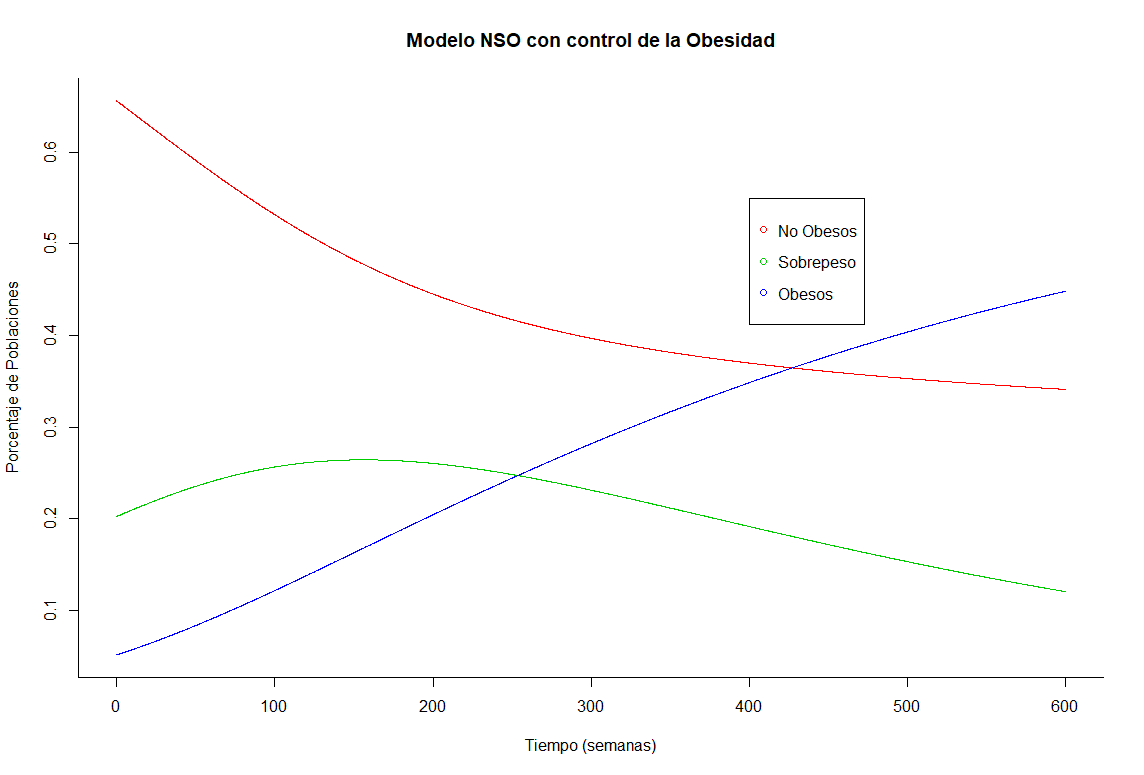
\includegraphics[scale=.30]{Control.png}%{NSO_nc.png}
	\caption{Uncontrolled model of obesity (\ref{eq:1})}
	\end{figure}
	
	
	It can be seen from the simulation of the model (\ref{eq:1}), that in a non-obese population of 100, 35 of those who are overweight and 25 obese, if the conversion rates to the subpopulations at risk are small , we will have control over obesity. Our purpose will be to demonstrate this situation theoretically.

	\section{Conclusiones}
	In this work, we analyze obesity from an epidemiological point of view. The first describes the propagation of two states of abnormality in weight of individuals, without considering any treatment.
	 
	 ...

	\section*{acknowledgment}
		%
	%\information
	%
	%\newpage
	\begin{thebibliography}{10}

%You can used the format lit.bib , but in this case use as a preamble: 
%   
%      \bibliographystyle{vancouver}
%    \bibliography{lit}


\bibitem{ar} Dawes J, González-Parra G, Rowley J. Enhancing the customer experience: contributions from information technology, J Business Res. 2005; 36(5):350-7.

\bibitem{ev} Evangelista A, Ortiz A, Ríos-Soto K, Urdapilleta A. {USA the fast food nation: Obesity as an epidemic.} Los Alamos National Laboratory; 2004.


\bibitem{ff} Abood S. Quality of improvement initiative in nursing homes[Internet]. Am J Nurs. 2002[Consultado 22 Nov 2012]; 102(6). Disponible en: http://www.nursingworld.org.


\bibitem{lo}   Romero S, Moreno FJ, Rodriguez IM.
 Linear Partial Differential Equations for Engineers and Scientists. 2th. ed. Boca Raton:  Chapman \& Hall/CRC; 2002.

\bibitem{th} Thomas D, Weedermann M, Fuemmeler B, Martin C, Dhurandhar N, Bredlau C, Bouchard C. Dynamic model predicting overweight, obesity, and extreme obesity prevalence trends. Obesity. 2014;  22(2):590-597.

\end{thebibliography}

\bigskip



\appendix
	
	\mbox{}\\


\begin{remark}
	


 \begin{proof} 
body of the environment  proof 
 finish with 
 \fin 
 \begin{verbatim}(\fin)
\end{verbatim}

\end{proof}

\end{remark}


\end{document}
